\documentclass{article}
\usepackage[margin=2cm]{geometry}
\usepackage{amsmath} % for math notation
\usepackage{enumerate} % for customizing lists
\usepackage{mathtools}
\usepackage{listings}
\usepackage[T1]{fontenc}
\usepackage{tikz}
\usepackage{graphicx}
\usepackage{float}
\usetikzlibrary{shapes,arrows}

\usepackage [english]{babel}
\usepackage [autostyle, english = american]{csquotes}

\title{COMP 4321 - Project}
\author{Leung Ka Wa, 20770807, kwleungau@connect.ust.hk}
\date{}

\begin{document}
    \maketitle
    \section*{Program code Structure}
        \subsection*{java source code (project\_package)}
            \begin{itemize}
                \item \textbf{Crawler.java} - Crawler class
                \item \textbf{StopStem.java} - StopStem class
                \item \textbf{URLIndex.java} - URLIndex class, use to manipulate the URL.db
                \item \textbf{WordIndex.java} - WordIndex class, use to manipulate the WordDB.db
                \item \textbf{Tester.java} - Tester class, use to test and run the crawler.
                \item \textbf{SearchEngine.java} - SearchEngine class, use to perform IR.
            \end{itemize}
        \subsection*{Library}
            No extra library from lab is used in this project.

    \section*{Design of the jdbm database scheme}

    \subsection*{URL.db}
    It contain of 6 objects. Each of them is a HTree.
    \begin{itemize}
        \item \textbf{PageID} - Store the URL and its pageID. \\[0.4em]
        (\textbf{String})URL = (\textbf{UUID})pageID. Example:\\[0.4em]
        http://library.hkust.edu.hk/events/staff-workshops/ = b9275b04-58a1-3f4f-ab38-606e30a198a8 \\[0.4em]
        Design decision: A ID mapping. 

        \item \textbf{ParentToChilden} - Store the parent to children relationship. \\[0.4em]
        (\textbf{UUID})parentID = Vector$\langle$\textbf{UUID}$\rangle$(childID). Example:\\[0.4em]
        5ed456f8-36f3-3ca2-8451-62696e13f7fc = [b9275b04-58a1-3f4f-ab38-606e30a198a8, 9e4a5a31-dbb7-39d0-82ab-8d8b37595564, bd93a542-88ec-3b29-b739-9faf1ffc3bdc, \dots] \\[0.4em]
        Design decision: Can easily get the out link of a page for later use, e.g. PageRank, hub weight, authority weight and HITS.
        
        \item \textbf{ChildToParents} - Store the child to parents relationship. \\[0.4em]
        (\textbf{UUID})childID = Vector$\langle$\textbf{UUID}$\rangle$(parentID). Example:\\[0.4em]
        5ed456f8-36f3-3ca2-8451-62696e13f7fc = [b9275b04-58a1-3f4f-ab38-606e30a198a8, 9e4a5a31-dbb7-39d0-82ab-8d8b37595564, bd93a542-88ec-3b29-b739-9faf1ffc3bdc, \dots] \\[0.4em]
        Design decision: Can easily get the in link of a page for later use, e.g. PageRank, hub weight, authority weight and HITS.

        \item \textbf{PageToTitle} - Store the pageID and its originial title. \\[0.4em]
        (\textbf{UUID})pageID = (\textbf{String})title. Example:\\[0.4em]
        bd93a542-88ec-3b29-b739-9faf1ffc3bdc = "This is the Title"\\[0.4em]
        Design decision: Store the whole title for display use only.

        \item \textbf{LastModified} - Store the pageID and its last modified date. \\[0.4em]
        (\textbf{UUID})pageID = (\textbf{Date})lastModifiedDate. Example:\\[0.4em]
        bd93a542-88ec-3b29-b739-9faf1ffc3bdc = (\textbf{Date})Thu Jun 16 16:47:33 HKT 2022\\[0.4em]
        Design decision: Store the last modified date of a page to determine whether the page is updated or not.
        
        \item \textbf{PageSize} - Store the pageID and its size. \\[0.4em]
        (\textbf{UUID})pageID = (\textbf{Integer})size. Example:\\[0.4em]
        bd93a542-88ec-3b29-b739-9faf1ffc3bdc = 1024\\[0.4em]
        Design decision: Store the size of a page to determine how much infomation are in this page.
    \end{itemize}


    \subsection*{WordDB.db}
    It contain of 4 objects. Each of them is a HTree.
    \begin{itemize}
        \item \textbf{WordID} - Store the word and its ID. \\[0.4em]
        (\textbf{String})word = (\textbf{UUID})wordID. Example:\\[0.4em]
        intellig = b9275b04-58a1-3f4f-ab38-606e30a198a8 \\[0.4em]
        Design decision: A ID mapping.
        \item \textbf{Inverted} - Store the wordID and posting list. \\[0.4em]
        (\textbf{UUID})wordID = Map$\langle$(\textbf{UUID})pageID, Vector$\langle$\textbf{Integer}$\rangle$(position)$\rangle$.
        Example:\\[0.4em]
        b9275b04-58a1-3f4f-ab38-606e30a198a8 = \{9bfc960c-53e4-3faf-8623-b44c251584c1=[1, 5, 10], 114471e0-e3dd-39d8-aa8a-11f77c85a7fa=[50, 60], 8019de9c-bcf5-3600-814b-53ed90ab33bb=[10], \dots \}\\[0.4em]
        Design decision: Store the posting list of the word for tfxidf and phase search. Also, finding the document with highest word frequency is easy.
        \item \textbf{Forward} - Store the pageID and its forward word list. \\[0.4em]
        (\textbf{UUID})pageID = Map$\langle$(\textbf{UUID})wordID, Vector$\langle$\textbf{Integer}$\rangle$(position)$\rangle$.
        Example:\\[0.4em]
        b9275b04-58a1-3f4f-ab38-606e30a198a8 = \{9bfc960c-53e4-3faf-8623-b44c251584c1=[1, 5, 10], 114471e0-e3dd-39d8-aa8a-11f77c85a7fa=[50, 60], 8019de9c-bcf5-3600-814b-53ed90ab33bb=[10], \dots \}\\[0.4em]
        Design decision: Store the forward word list of the page for later algorithm, e.g. tfxidf. Finding the words and their position to get the phase and frequency in a document is easy.
        \item \textbf{TitleInverted} - Store the wordID and posting list of title. \\[0.4em]
        (\textbf{UUID})wordID = Map$\langle$(\textbf{UUID})pageID, Vector$\langle$\textbf{Integer}$\rangle$(position)$\rangle$.
        Example:\\[0.4em]
        b9275b04-58a1-3f4f-ab38-606e30a198a8 = \{9bfc960c-53e4-3faf-8623-b44c251584c1=[1, 5, 10], 114471e0-e3dd-39d8-aa8a-11f77c85a7fa=[50, 60], 8019de9c-bcf5-3600-814b-53ed90ab33bb=[10], \dots \}\\[0.4em]
        Design decision: Store the posting list of the word in title to favor matches in title.
    \end{itemize}

    \newpage
    \section*{Running the program (crawler part)}
    \subsection*{How to run the program}
    
        The Tester class is the main calling class of this program. Pass command line argument to it to run the program. \\[0.4em]
        As I am using VS code to develop this project, I was just simply using the java extension and run the program without mannually compile the project. 
        For me the command line is:
        \begin{lstlisting}[language=bash,breaklines=true]
            /usr/bin/env /Users/boscoleung/opt/anaconda3/bin/java @/var/folders/f1/6mvnwxt109n9rswystbch0t40000gn/T/cp_dh97avm16bvprxybpew6los8v.argfile project_package.Tester <argument>
        \end{lstlisting}

        If you want to compile the project mannually, you can run the following command (work on mac): \\[0.8em]
        % \centerline{\textbf{javac -cp \texttt{"}:lib/*\texttt{"} -d bin \$(find . -name \texttt{"}*.java\texttt{"})}} 
        \centerline{\textbf{javac -cp \texttt{"}:lib/*\texttt{"} -d bin \$(find . -path ./apache-tomcat-10.1.6 -prune -o -name \texttt{"}*.java\texttt{"} -print)}} \\[0.1em]

        A bin folder containing all the classes will be created.
        \begin{figure}[!htbp]
            \centering
            \caption{The complied bin folder}
            \label{}
            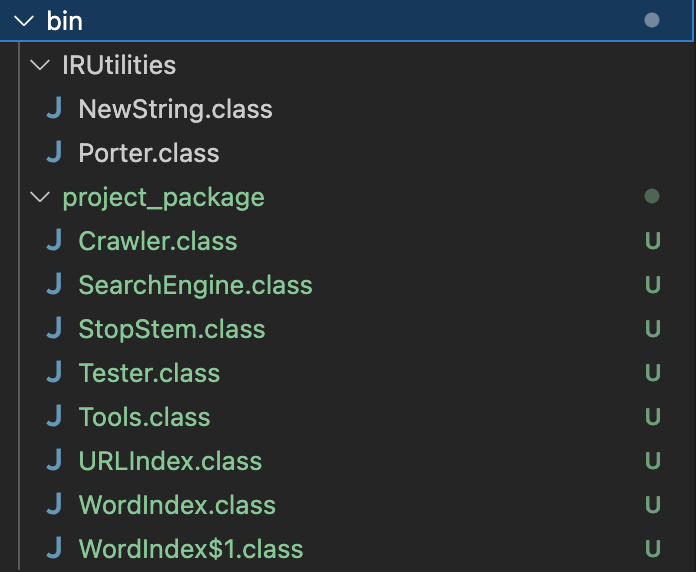
\includegraphics[width=5cm]{compliedBin.png}
        \end{figure}

        Then run the program with the following command: \\[0.8em]
        \centerline{\textbf{java -cp \texttt{"}.:bin:lib/*\texttt{"} project\texttt{\_}package.Tester $<$argument$>$}}

        \begin{itemize}
            \item \textbf{-runCrawler} - Run the crawler, progress will be printed to the console. The starting URL and the number of pages to crawl can be set by add the url and number. For example, \textbf{\texttt{-runCrawler https://www.google.com 1000}}, if no url and number is provided, the default url and number will be used, that is \textbf{\texttt{-runCrawler} $=$ \texttt{-runCrawler https://www.cse.ust.hk/$\sim$kwtleung/COMP4321/testpage.htm 300}};
            \item \textbf{-printSpiderResult} - Output the result of the crawler to spider\_result.txt. This may take a moment to produce the complete result.
            \item \textbf{-printAllURLdb} - Output all the data in the URL.db to AllURLdb.txt.
            \item \textbf{-printPageTitle} - Output all the data in the URL.db PageToTitle to PageTitle.txt.
            \item \textbf{-printURLPageID} - Output all the data in the URL.db PageID to URLPageID.txt.
            \item \textbf{-printPageMeta} - Output all the data in the URL.db LastModified and PageSize to PageMeta.txt.
            \item \textbf{-printParentToChilden} - Output all the data in the URL.db ParentToChildren to ParentToChildren.txt.
            \item \textbf{-printChildToParents} - Output all the data in the URL.db ChildToParents to ChildToParents.txt.
            \item \textbf{-printAllWordDB} - Output all the data in the WordDB.db to AllWordDB.txt.
            \item \textbf{-printWordID} - Output all the data in the WordDB.db WordID to WordID.txt.
            \item \textbf{-printInverted} - Output all the data in the WordDB.db Inverted to Inverted.txt.
            \item \textbf{-printTitleInverted} - Output all the data in the WordDB.db TitleInverted to TitleInverted.txt.
            \item \textbf{-printForward} - Output all the data in the WordDB.db Forward to Forward.txt.
        \end{itemize}

    % Define block styles
    \tikzstyle{decision} = [diamond, draw, fill=blue!20, 
    text width=5em, text badly centered, node distance=3cm, inner sep=0pt]
    \tikzstyle{block} = [rectangle, draw, fill=blue!20, 
    text width=8em, text centered, rounded corners, minimum height=2.5em]
    \tikzstyle{line} = [draw, -latex']
    \tikzstyle{cloud} = [draw, ellipse,fill=red!20, node distance=3cm,
    minimum height=2em]
    
    \newpage
    \section*{Search Engine Design}
    \begin{center}
        \begin{tikzpicture}[node distance = 2cm, auto]
            % Place nodes
            \node [cloud] (input) {input query};
            \node [block, below of=input, node distance=1.5cm, text width=10em] (stomstem) {stop stem every word};

            \node [block, below of=stomstem, text width=35em, node distance=2cm, left] (queryTerm) {calculate query term weight (phase consider as a term) \\
            $w_{term,query}=(0.5+0.5\frac{tf_{term,query}}{max(tf_{query})})\log_2(1+\frac{N_{num\_indexed\_page}}{df_{num\_page\_contain\_term}})$ \\
            noraml query word that havent appear in the database will be ignored.};
            
            \node [block, below of=stomstem, right=1cm, node distance=2cm, text width=10em] (queryTermException) {if $df_{phase\_word}=0$ \\ Or all the query words havent appear in the database};

            \node [cloud, below of=queryTermException, node distance=3cm] (noResultEndding) {No Result};

            \node [decision, below of=queryTerm, , node distance=2.75cm] (phaseDecide) {contain phase search?};


            \node [block, left of=phaseDecide, node distance=4cm] (phaseSearch) {phase search};
            \node [block, below of=phaseSearch, text width=20em] (processPhaseSearch1) {obtain the page that contain the phase word with count in body and title respectively};
            \node [block, below of=processPhaseSearch1, text width=20em, node distance = 1.8cm] (processPhaseSearch2) {calculate the term weight of the page\\ $w_{term,page}=(0.5+0.5\frac{tf_{term,page}}{max(tf_{page})})\times$ \\ $\log_2(1+\frac{N_{num\_indexed\_page}}{df_{num\_page\_contain\_term}})$\\ Zero if the term havent appear in the page};
            \node [block, below of=processPhaseSearch2, text width=20em, node distance=2.2cm] (processPhaseSearch3) {favor query word in title by frequency:\\ $w_{term}=w_{term,page}\times(1.5\times tf_{term\_in\_title,page})$};

            \node [block, below of=processPhaseSearch3, text width=20em, node distance=1.5cm] (processPhaseSearch4) {favor phase word in body by frequency:\\ $w_{phase}=w_{phase,page}\times(1.25\times tf_{phase,page})$};

            \node [block, below of=processPhaseSearch4, text width=20em, node distance=1.5cm] (processPhaseSearch5) {favor phase word in title by frequency:\\ $w_{phase,page}=w_{phase,page}\times(3\times tf_{phase\_in\_title,page})$};



            \node [block, right of=phaseDecide, node distance=4cm] (normalSearch) {normal search};
            \node [block, below of=normalSearch, text width=20em, node distance = 2.5cm] (processNormalSearch1) {calculate the term weight of the page\\ $w_{term}=(0.5+0.5\frac{tf_{term,page}}{max(tf_{page})})\times$ $\log_2(1+\frac{N_{num\_indexed\_page}}{df_{num\_page\_contain\_term}})$ \\ Zero if the term havent appear in the page};

            \node [block, below of=processNormalSearch1, text width=20em, node distance = 2.5cm] (processNormalSearch2) {favor query word in title by frequency:\\ $w_{term}=w_{term,page}\times(1.5\times tf_{term\_in\_title,page})$};

            \node [block, below of=phaseDecide, text width=25em, node distance = 11.1cm] (pageWeight) {calculate the pages weight:\\ $w_{page}=\sum_{term\in query}w_{term,query}\times w_{term,page}$};

            \node [block, below of=pageWeight, text width=25em,, node distance = 1.5cm] (normalize) {normalize the page score:\\ $score_{page}=\log_2(w_{page})$};

            \node [block, below of=normalize, text width=25em, node distance = 1.5cm] (sort) {sort the page by score and \\ return \{(UUID)page1=$score_{page1}\dots$\}};

            \node [cloud, below of=sort, node distance = 1.5cm] (output) {output the result};
            
            % Draw edges
            \path [line] (input) -- (stomstem);
            \path [line] (stomstem) -- (queryTerm);
            \path [line] (queryTerm) -- (phaseDecide);
            \path [line,dashed] (queryTerm) -- (queryTermException);
            \path [line] (queryTermException) -- (noResultEndding);
            
            \path [line] (phaseDecide) -- node {yes} (phaseSearch);
            \path [line] (phaseSearch) -- (processPhaseSearch1);
            \path [line] (processPhaseSearch1) -- (processPhaseSearch2);
            \path [line] (processPhaseSearch2) -- (processPhaseSearch3);
            \path [line] (processPhaseSearch3) -- (processPhaseSearch4);
            \path [line] (processPhaseSearch4) -- (processPhaseSearch5);
            \path [line] (processPhaseSearch5) -- (pageWeight);

            \path [line] (phaseDecide) -- node {no} (normalSearch);
            \path [line] (normalSearch) -- (processNormalSearch1);
            \path [line] (processNormalSearch1) -- (processNormalSearch2);
            \path [line] (processNormalSearch2) -- (pageWeight);

            \path [line] (pageWeight) -- (normalize);
            \path [line] (normalize) -- (sort);
            \path [line] (sort) -- (output);

        \end{tikzpicture}
    \end{center}

    \section*{Running the user interface (JSP web)}

    \newpage
    \section*{Bonus features beyond requirement}
        \subsection*{Query length}
            The query length don't have a maximum. It can be any length.    
        \subsection*{Phase length}
            The phase length is not limited to 2 or 3. It can be any length. Of course, the longer the phase, the less the result contain matches.
        
        \subsection*{Query weight}
            The query weight is not 1. It is calculated by the following formula:
            \begin{equation*}
                w_{term,query}=\frac{tf_{term,query}}{max(tf_{query})}\times\log_2(1+\frac{N_{num\_indexed\_page}}{df_{num\_page\_contain\_term}})
            \end{equation*}
            Therefore, it can show the importance of the term in the query. For example, a search query 'definition of quantum in quantum mechanics', the term $tf$ part of the term 'quantum' will be larger than others. Which can show the different of importance level in the query.

        \subsection*{Fast crawling speed}
            The crawler can crawl 1000 pages in 1 minute. The speed is fast enough for the search engine.

        \subsection*{Additional crawler in JSP web interface to index more pages}

    \newpage
    \section*{Conclusion}

    \newpage
    \section*{Special Notice}
        \subsection*{Word Extraction}
            I have set 
            \begin{lstlisting}[language=Java]
                sb.setLinks(false)
            \end{lstlisting} 
            in the word extraction part, which is different from the lab. \\[0.4em] 
            Since if it is set to true, it will create some keywords like $httpslibraryhkusteduhkaboutushoursservicepointshoursservic$ and $httpslibraryhkusteduhkhelpforalumnialumni$, it doesn't seem to make sense. 
        \subsection*{Crawler Strategy}
            I have implemented the BFS strategy in this phase. And the crawler will pick the next URL according the occurrence order in the webpage.
        \subsection*{Page Last Modified Date and Page Size}
            Currently I am using the following method to get the last modified date of the page:
            \begin{lstlisting}[language=Java]
                url.openConnection().getLastModified();
            \end{lstlisting}
            But it seems that the last modified date may missing. In this case, the last modified date will be set to 
            \begin{lstlisting}[language=Java]
                url.openConnection().getDate();
            \end{lstlisting}
            which is the date of accessing. \\[0.4em]
            For the page size, I am using the following method to get the page size:
            \begin{lstlisting}[language=Java]
                url.openConnection().getContentLength();
            \end{lstlisting}
            If the page size is missing, I will use the page size value method obtain in lab 2 instead.
        
            
\end{document}